\documentclass{article}

% Package Declarations
\usepackage{arxiv}
\usepackage[utf8]{inputenc} % allow utf-8 input
\usepackage[T1]{fontenc}    % use 8-bit T1 fonts
\usepackage{hyperref}       % hyperlinks
\usepackage{url}            % simple URL typesetting
\usepackage{booktabs}       % professional-quality tables
\usepackage{amsfonts}       % blackboard math symbols
\usepackage{nicefrac}       % compact symbols for 1/2, etc.
\usepackage{microtype}      % microtypography
\usepackage{lipsum}         % Lorem Ipsum fill text
\usepackage{multicol}       % Support for Multi columns for tables
\usepackage{multirow}       % Support for Multi rows fot tables
\usepackage{mathtools}      % Advanced mathtools
\usepackage{caption}        % Advanced caption configuration
\usepackage{amsmath}        % Math package for equations       
\usepackage{titlesec}       % Title section
\usepackage{graphicx}       % For adding labels to parts of the equation
\usepackage{stackrel}       % For adding labels to parts of the equation

% Theme Configurations

% Set section depth to 4
% \setcounter{secnumdepth}{4}

% \titleformat{\paragraph}
% {\normalfont\normalsize\bfseries}{\theparagraph}{1em}{}
% \titlespacing*{\paragraph}
% {0pt}{3.25ex plus 1ex minus .2ex}{1.5ex plus .2ex}

% Add padding to text below table
\captionsetup[table]{skip=10pt}

% Configure hat tex
\let\oldhat\hat
\renewcommand{\hat}[1]{\oldhat{\mathbf{#1}}}

% Document Start

\title{Differentiable Learning by means of Neural Network Pruning}

\author{
  Prathyush S Parvatharaju\thanks{Use footnote for providing further
    information about author (webpage, alternative
    address)---\emph{not} for acknowledging funding agencies.} \\
  Department of Data Science\\
  Worcester Polytechnic University\\
  Worcester, MA 01609 \\
  \texttt{psparvatharaju@wpi.edu} \\
  %% examples of more authors
   \And
 Shreesha Narasimhamurthy \\
  Department of Data Science\\
  Worcester Polytechnic University\\
  Worcester, MA 01609 \\
  \texttt{snarasimhamurthy@wpi.edu} \\
}

\begin{document}
\maketitle

\begin{abstract}
The idea of linear flow i.e, each node in one layer is connected to a certain weight $\hat{W_{ij}}$ to every node in the following layer, for the deep neural network is limiting in the sense of the way we, humans think. The linear flow would be a constraint for a DNN as the later can process data and emulate relationships in higher dimensions. Deeper neural networks are difficult to train and the use of residual learning \cite{He2016DeepRL} in the form of short-circuit connections eases the process of training the network. By replacing the linear flow constraint with a decision process of placing short-circuit connections between layers as a gradient-based approach would yield better results. We propose a novel idea of extending the capabilities of previously used short-circuits as differentiable functions, \cite{Trask2018NeuralAL}, essentially solving “What to feed?”. To tackle the problem, “When to stop?” we propose an algorithm based on Information Transfer derived from differentiable short-circuits. 

In our experiments we showcase that increased weighted representation capability results in achieving better accuracy in fewer iterations compared to the standard architecture. We also demonstrate that even with 10\% of the previous parameters, the architecture achieves similar results to standard architecture. Another set of experiments shows our proposed architecture can build better representations with minimal data.
\end{abstract}


% keywords can be removed
\keywords{Differentiable Learning \and Pruning \and Neural Architecture Search}


\section{Introduction}
The ability to recognize patterns and develop strong relations among them has made Neural Network supersede state of the art machine learning techniques. The depth of representations is of central importance for many visual recognition tasks. Right from Alex Net \cite{Krizhevsky2012ImageNetCW} up until ResNet \cite{He2016DeepRL} the flow of data followed linear fashion i.e the data flows from one layer to the next layer and so on. ResNet brought in an innovation \emph{"Short Circuits"} meaning there exists a skip connection where the data is fed to the next layer and in certain circumstances it is fed to next layer and also the layer after its immediate next. This paved way to train deep-networks as it increased the representational capability of the network by overcoming issues such as vanishing / exploding gradients \cite{Bengio1994LearningLD, Glorot2010UnderstandingTD}. In our work we set out a goal to explore the \emph{"representational capability"} and its effects on the performance of the network. This led to the question - "What to feed?".

ResNet brings in short circuits between residual components and the number of skip connections are restricted. We propose \emph{"Global Short Circuit"}(GSC) to investigate the behaviour of short circuits by revoking the restriction and providing skip connections from one layer to every other layer. This enhances representational capability of the network and results in achieving better accuracy in fewer iterations compared to standard architecture (See section \ref{sssec:ffn}). However, the modification results in a large network compared to a standard architecture. Due to increased parameters, the network is not scalable. To tackle this issue we propose an enhanced GSC i.e\emph{"Differentiable Short Circuit"}(DSC) - a novel architecture to help network scale by pruning unwanted skip connections over time.

To tackle the issue of \emph{"When to stop"}?, we devise an algorithm - \emph{Information Transfer}. It is a measure of the amount of flow of data from one layer to another. By keeping track of variance in the Information Transfer over iterations, based on a certain threshold we propose a stoping criteria.

\section{Differentiable Learning}
\label{sec:headings}

Neural networks are differentiable by design. The standard architecture (\ref{sssec:ffn}) is static and does not change over time whereas the learning changes over time. There have been efforts towards an automated way of finding the best architecture for the given data - Neural Architecture search \cite{Zoph2016NeuralAS}. With the recent advent of DARTS \cite{Liu2019DARTSDA} shows that a learning based adaptive architecture performs better compared to a static architecture. Given $N$ layers, we need to find the optimal data paths. We can find the right set of combinations by using brute-force is to try out n(n-1) combinations of connection configurations. However as the depth of the network increases, the search space increases exponentially and training each configuration becomes a tedious and time consuming effort. Gradient descent \cite{ruder2016overview} - a first order iterative search space optimization algorithm finds the local minimum of a differentiable function. In order to find the right connections, we represent connection as a differentiable function and find $\frac{\partial loss}{\partial connection}$. We first describe a standard architecture - Feed forward neural network and propose Global short circuit (GSC) and Differentiable Short Circuit (DSC) architectures.

\subsection{Feed Forward Neural Network}
\label{sssec:ffn}
Multilayer perceptron trained using back-propagation \cite{Rumelhart1986LearningIR}, a supervised learning algorithm are useful for their ability to solve the problems stochastically often approximating solutions for complex problems. Acting as a universal approximator, the architecture has a linear flow. The current layer take only the output of previous layer as input. Since the number of connections increase linearly based on the nodes in the layer, the architecture is scalable and time efficient. Figure \ref{fig:SimpleFFN.png} represents standard feed forward architecture and equation \ref{eq:ffn_math_representation} is the mathematical formulation of the network. Each node in one layer is connected to a certain weight $\hat{W_{ij}}$ to every node in the following layer. 

\begin{equation}
\label{eq:affine_transformation}
\begin{aligned}
\hat{Z} &= Input \cdot \hat{W} + \hat{b}&\\
\end{aligned}
\end{equation}

A squashing non-linear transformation $\sigma$ \cite{Han1995TheIO} is applied to output of each node.

\begin{equation}
\label{eq:sigmoid_activation}
\begin{aligned}
\sigma(x) &= \frac{1}{1+e^-x} \;\;\;\;\;\;  x\in\mathbb{R}, 0<\sigma(x)<1
\end{aligned}
\end{equation}

\noindent\begin{minipage}{.45\textwidth}
   \centering
   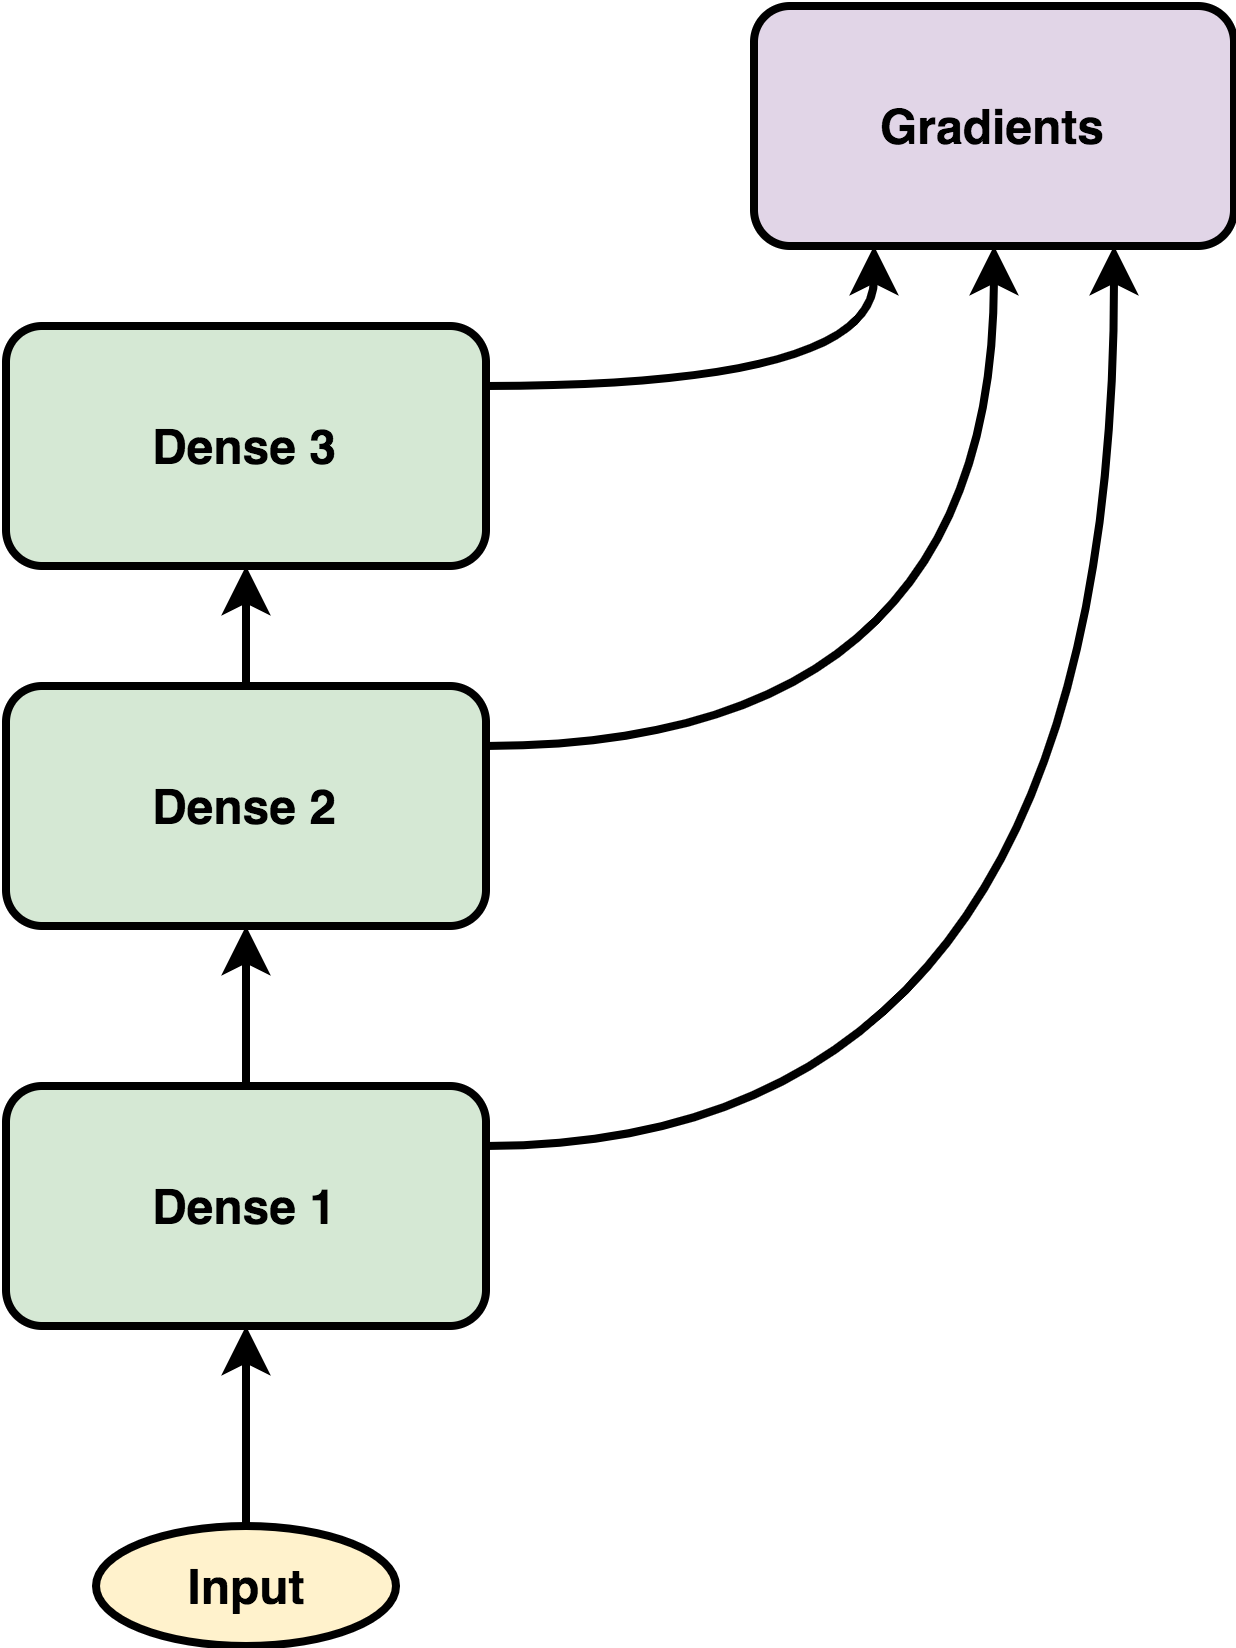
\includegraphics[scale=0.09]{SimpleFFN.png}
   \captionof{figure}{Feed Forward Network}
   \label{fig:SimpleFFN.png}
\end{minipage}
\begin{minipage}{.45\textwidth}
\begin{equation}
\label{eq:ffn_math_representation}
\begin{aligned}
   Dense_{1} &= \sigma(Input \cdot \hat{W}_{1} + \hat{b}_{1}) &\\
   Dense_{2} &= \sigma(Dense_{1} \cdot \hat{W}_{2} + \hat{b}_{2}) &\\
   Dense_{3} &= \sigma(Dense_{2} \cdot \hat{W}_{3} + \hat{b}_{3}) 
\end{aligned}
\end{equation}
\end{minipage}

The number of trainable parameters for a current layer is only a function of the layer's weight, bias and input. It can be represented as, 

\begin{equation}
\label{eq:ffn_params}
Params= \sum_{n=1}^{m}
\underbrace{(L_{n-1}\rule[-12pt]{0pt}{5pt}}_{\mbox{input}}
*\underbrace{L_{n})\rule[-12pt]{0pt}{5pt}}_{\mbox{weights}}
+\underbrace{L_{n}\rule[-12pt]{0pt}{5pt}}_{\mbox{bias}}
\end{equation}

For a 3 layer network with node configurations [100,50,10] and 784 input features, using equation \ref{eq:ffn_params} we arrive at 83,550 trainable parameters


\vspace{2em}

\subsection{Global Short Circuit}
We propose Global Short Circuit architecture to explore the impact of skip connection on representational capabilities of the network. There exists a connection from every layer to every other layer in the network. Few possible ways of merging layers are explored in DenseNet\cite{Li2018DenselyCC} and ResNet\cite{He2016DeepRL}. In ResNet weighted feature maps are merged using $max$ or $sum$. DenseNet merges feature using a concatenate operation. We define a merge operation similar to DenseNet - $concat$ style merge. However this style of merge has an issue when it comes to Convolutional Neural Networks where there is a requirement to merge feature maps of different shapes. We use downsampling/padding operators to get identical shapes. Figure \ref{fig:GSC.png} shows standard architecture defined in section \ref{sssec:ffn} having connections from one layer to every other layer, merged using concat operation. Equation \ref{eq:gsc_math_representation} provides mathematical representation of the architecture.

\noindent\begin{minipage}{.45\textwidth}
   \centering
   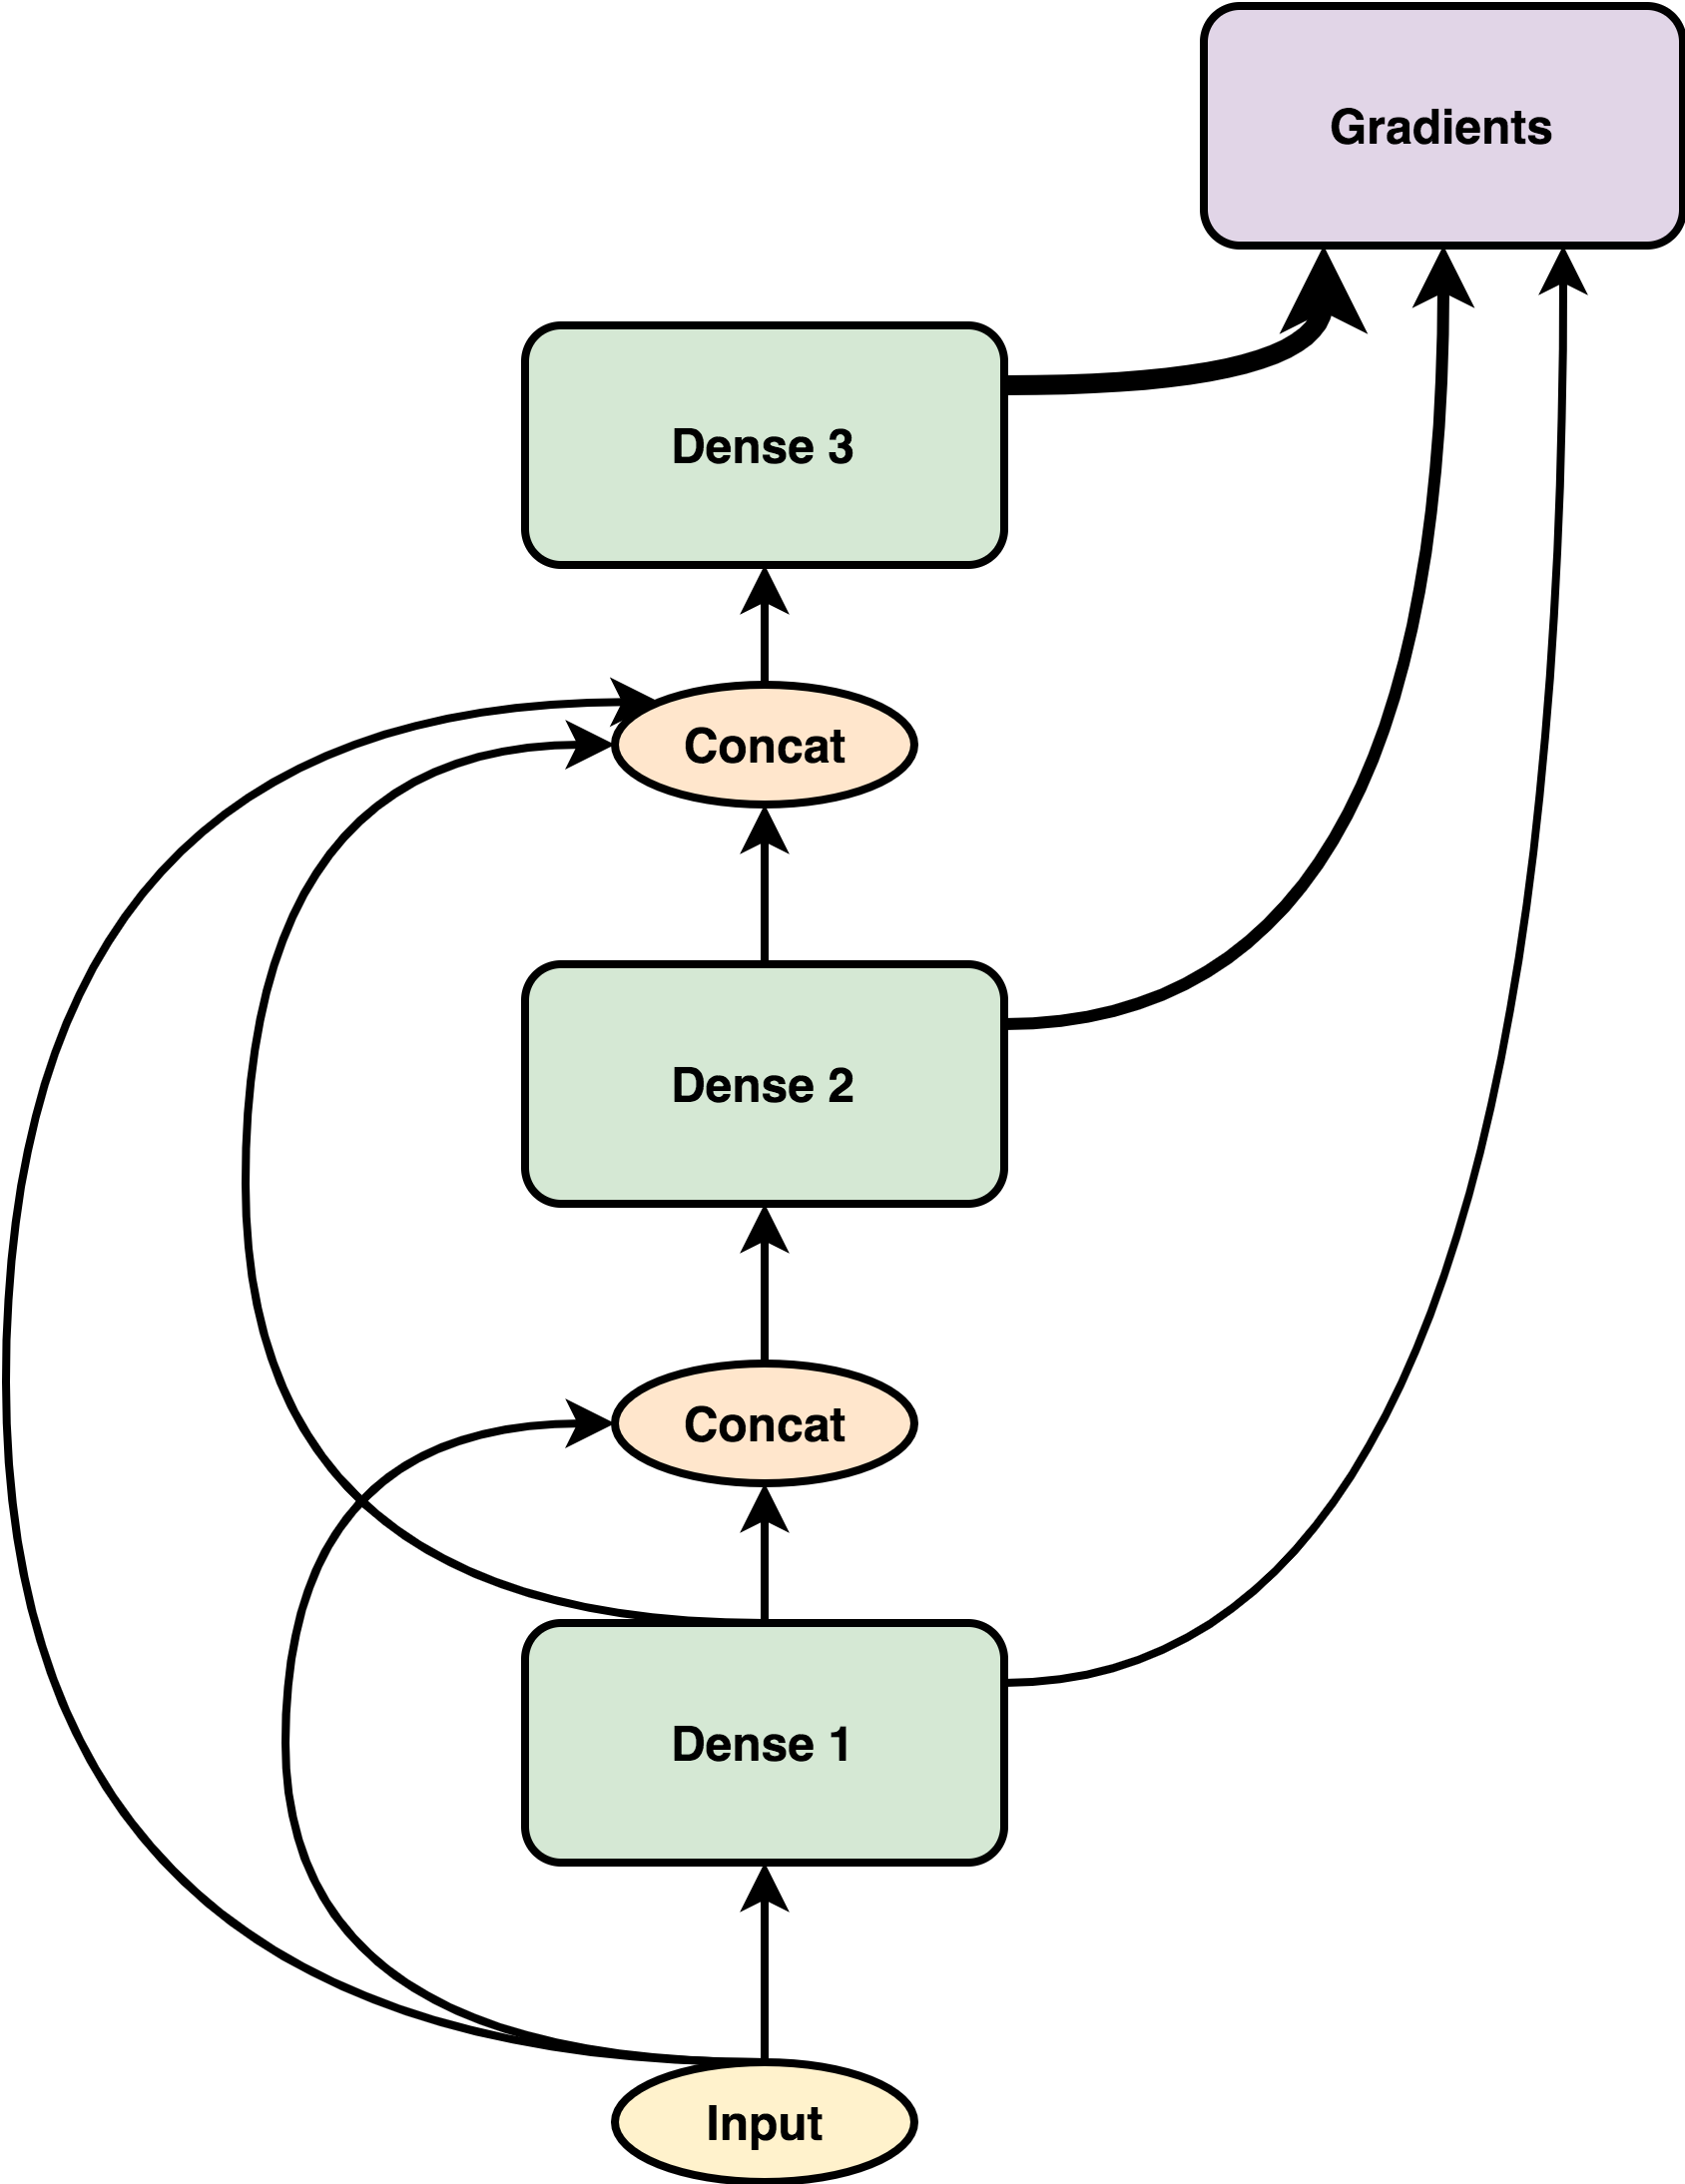
\includegraphics[scale=0.09]{GSC.png}
   \captionof{figure}{Global Short Circuit}
   \label{fig:GSC.png}
\end{minipage}
\begin{minipage}{.45\textwidth}
\begin{equation}
\label{eq:gsc_math_representation}
\begin{aligned}
       Dense_{1} &= \sigma(Input \cdot \hat{W}_{1} + \hat{b}_{1}) &\\
       Dense_{2} &= \sigma([Input \oplus Dense_{1}] \cdot \hat{W}_{2} + \hat{b}_{2}) &\\
       Dense_{3} &= \sigma([Input \oplus Dense_{1} \oplus Dense_{2}] \cdot \hat{W}_{3} + \hat{b}_{3}) 
\end{aligned}
\end{equation}
\end{minipage}

Experiments show that GSC performs better than standard architecture on large and minimal datasets. This is due to increased representational capacity of the network. A layer \emph{n} in the network now has access every other \emph{n-1} previous outputs. This change paves way to create much deeper constructs and complex relationships among the layers. However, it suffers from an exponential increase in connections resulting in delayed training times. As the complexity of the network increases in terms of depth, we notice a rise in the number of stacked layers and is not scalable.

Compared to the standard architecture, GSC has a considerable increase in the number of training parameters.  This is due to the effect of merge operation of previous $n-1$ layers for $n$th layer.

\begin{equation}
\label{eq:gsc_params}
Params= \sum_{n=1}^{m}\left[
\underbrace{(\sum_{i=0}^{n}L_{i}\rule[-12pt]{0pt}{5pt}}_{\mbox{merged inputs}}
*\underbrace{L_{n})\rule[-12pt]{0pt}{5pt}}_{\mbox{weights}}
+\underbrace{L_{n}\rule[-12pt]{0pt}{5pt}}_{\mbox{bias}}\right]
\end{equation}

For the previously mentioned 3 layer network, we have to train an exponential increase of 30\% i.e, 122,750 parameters.

\subsection{Differentiable Short Circuit}
\lipsum[6]
\lipsum[6]
\lipsum[6]
\lipsum[6]

\noindent\begin{minipage}{.45\textwidth}
   \centering
   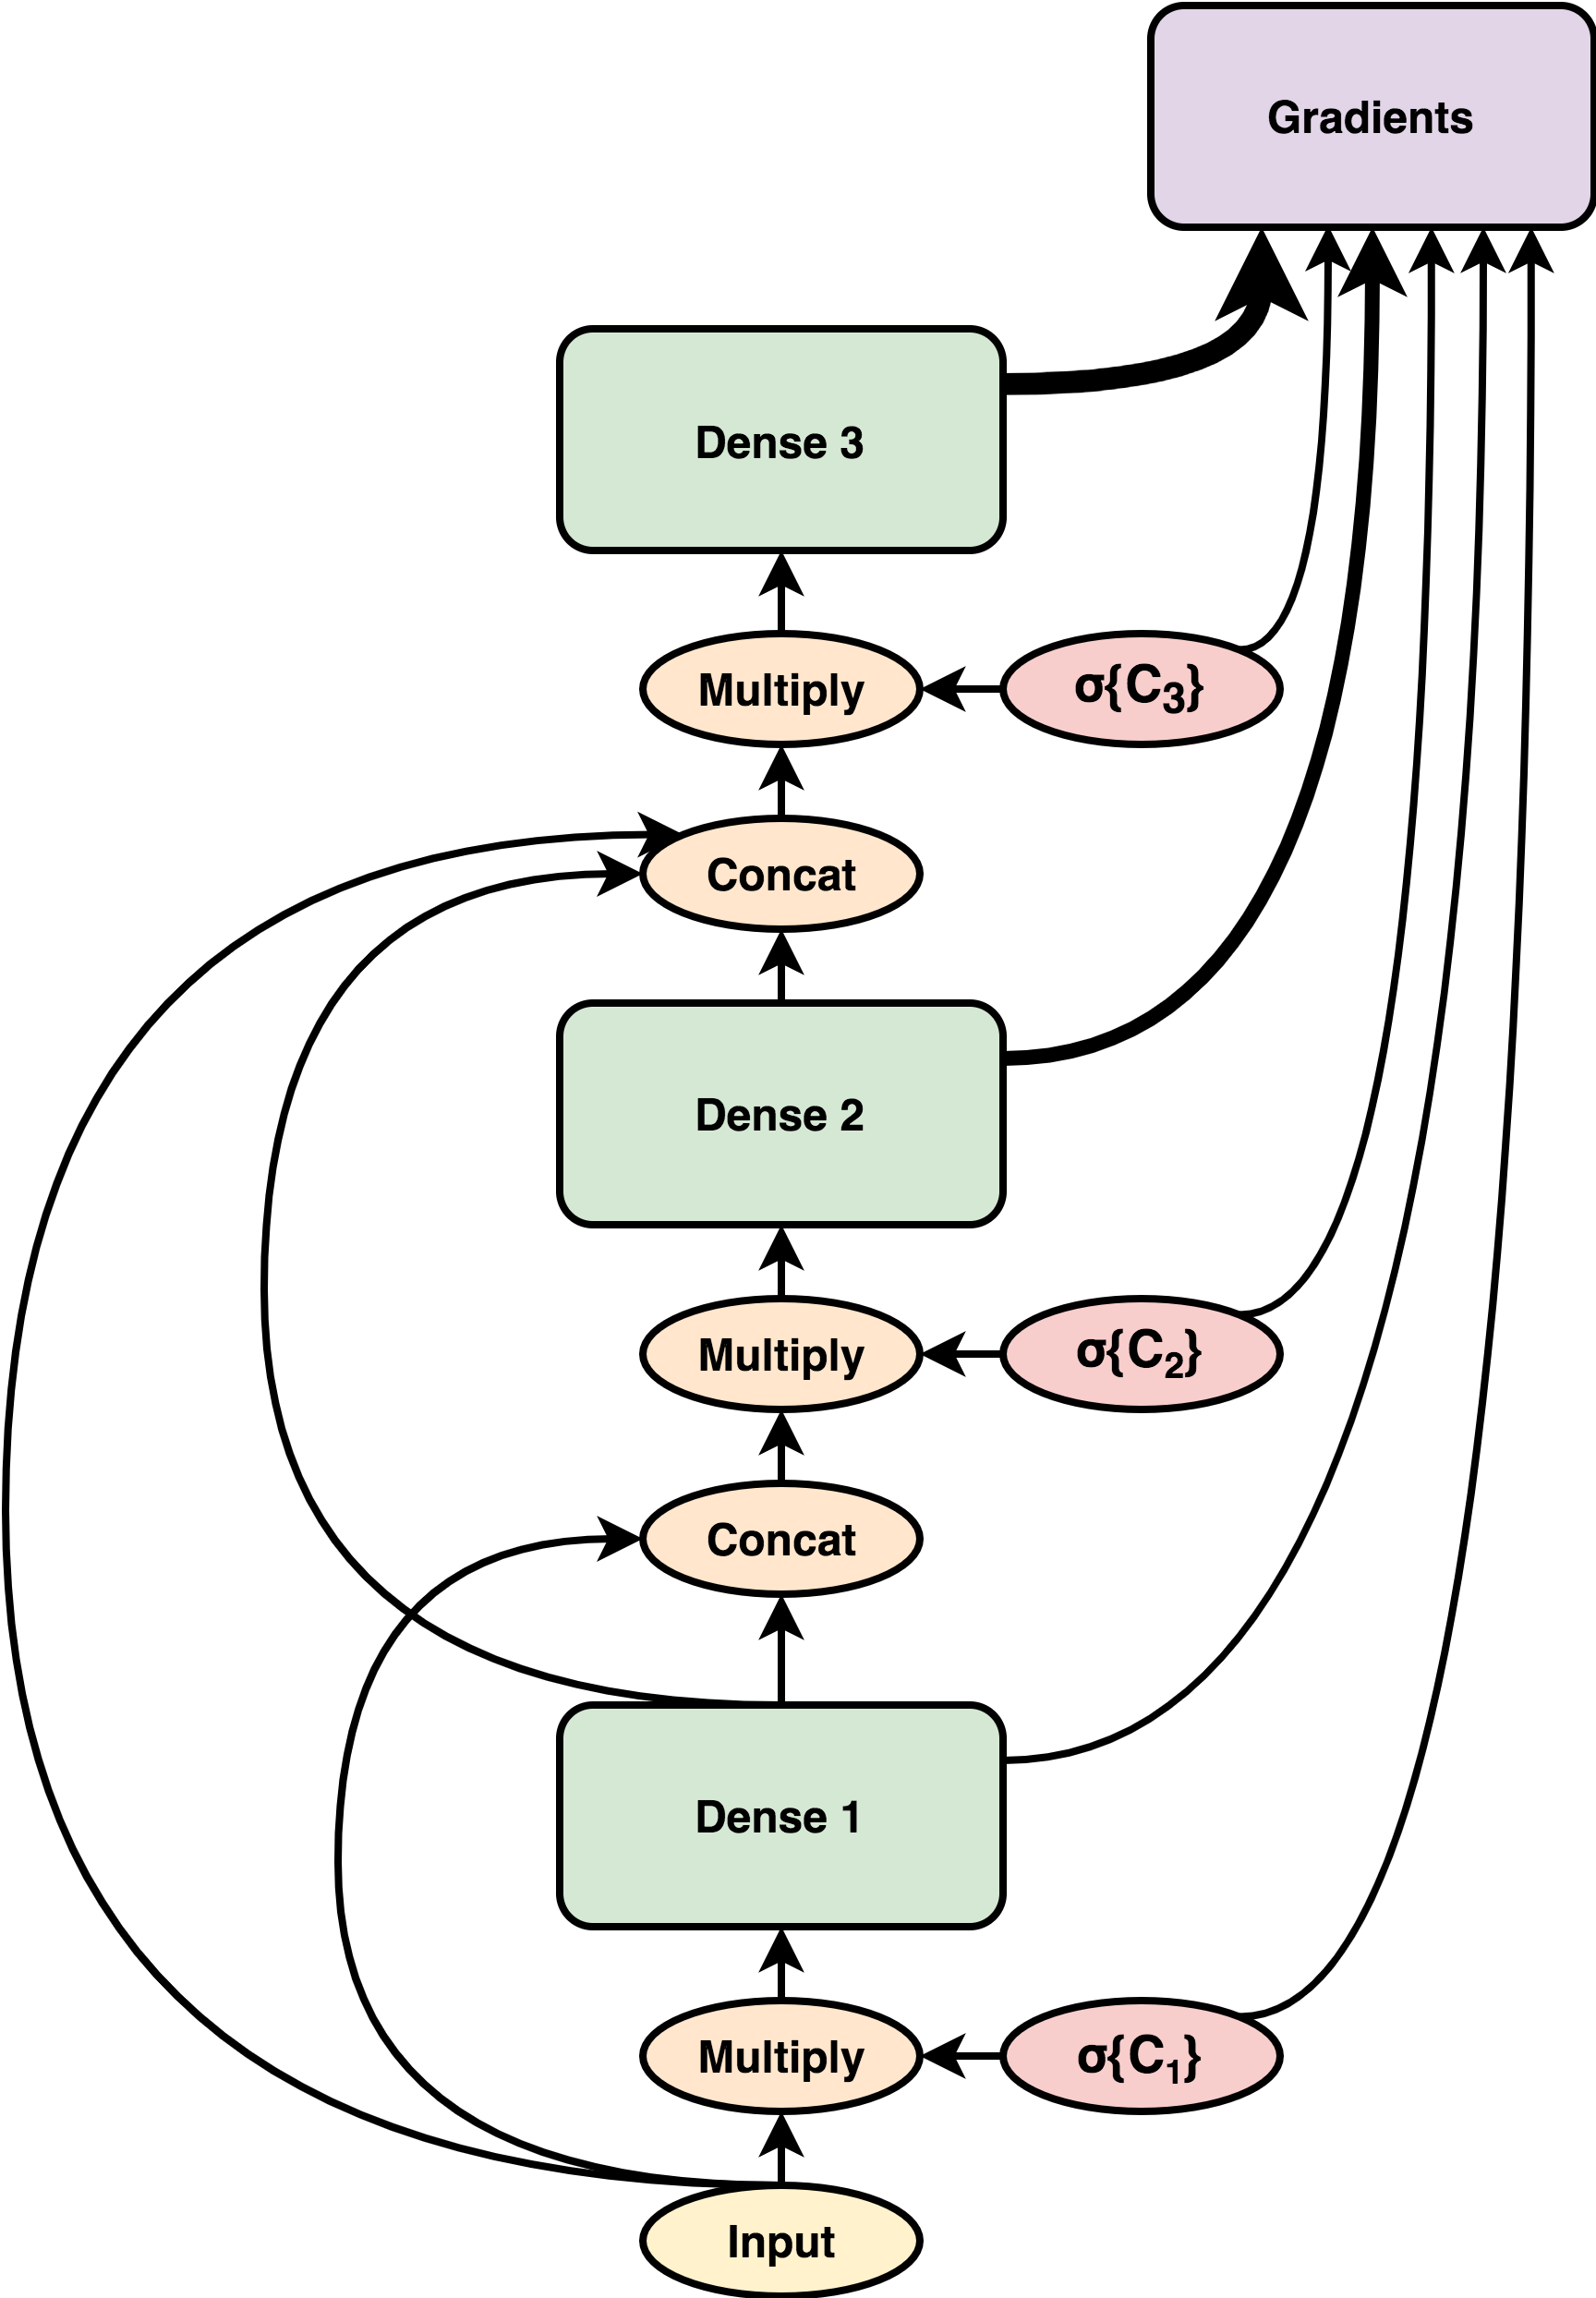
\includegraphics[scale=0.09]{DSC.png}
   \captionof{figure}{Differentiable Short Circuit}
   \label{fig:DSC.png}
\end{minipage}
\begin{minipage}{.45\textwidth}
\begin{equation}
\label{eq:ffn_math_representation}
\begin{aligned}
   Dense_{1} &= \sigma((\sigma(\hat{C}_{1}) \cdot Input) \cdot \hat{W}_{1} + \hat{b}_{1}) &\\
   Dense_{2} &= \sigma((\sigma(\hat{C}_{2}) \cdot [Input \oplus Dense_{1}]) \cdot \hat{W}_{2} + \hat{b}_{2}) &\\
   Dense_{3} &= \sigma((\sigma(\hat{C}_{3}) \cdot [Input \oplus Dense_{1} \oplus Dense_{2}]) \cdot \hat{W}_{3} + \hat{b}_{3}) 
\end{aligned}
\end{equation}
\end{minipage}

Comparing to equation \ref{eq:gsc_params} 

\begin{equation}
\label{eq:dsc_math_representation}
Params= \sum_{n=1}^{m}\left[
\underbrace{(\sum_{i=0}^{n}L_{i}\rule[-12pt]{0pt}{5pt}}_{\mbox{merged inputs}}
*\underbrace{L_{n})\rule[-12pt]{0pt}{5pt}}_{\mbox{weights}}
+\underbrace{L_{n}\rule[-12pt]{0pt}{5pt}}_{\mbox{bias}}
+\underbrace{\sum_{i=0}^{n}L_{i}\rule[-12pt]{0pt}{5pt}}_{\mbox{connection weights}}\right]
\end{equation}

For DSC we notice a slight increase in parameters due to the use \emph{gates}. There exists a trainable gate for every connection. As a result, for the network structure defined in the standard architecture, the number of trainable parameter is 124,418.

\subsubsection{Information Transfer}
We propose \emph{Information transfer} (IT) as the percentage of measure of data flow from one layer to the next. The gated connections having sigmoid activation \cite{Han1995TheIO} defined by $\sigma(x) = \frac{1}{1+e^-x}$ $x\in\mathbb{R}, 0<\sigma(x)<1$  gives the ability to express the transfer in terms of percentage. 

\noindent\begin{minipage}{.45\textwidth}
\begin{align*}
  IT &=\frac{\sum_{c=1}^{N}\hat{W}_{c}}{\sum_{c=1}^{N}|\hat{W}_{c}|}, \\
  \\
  \text{where}~N &= \text{Number of layers,} \\
  \hat{W}_{c} &= \text{Connection weight}\\
  |\hat{W}_{c}| &= \text{Length of connection weight}\\
\end{align*}
\end{minipage}
\begin{minipage}{.45\textwidth}
   \centering
   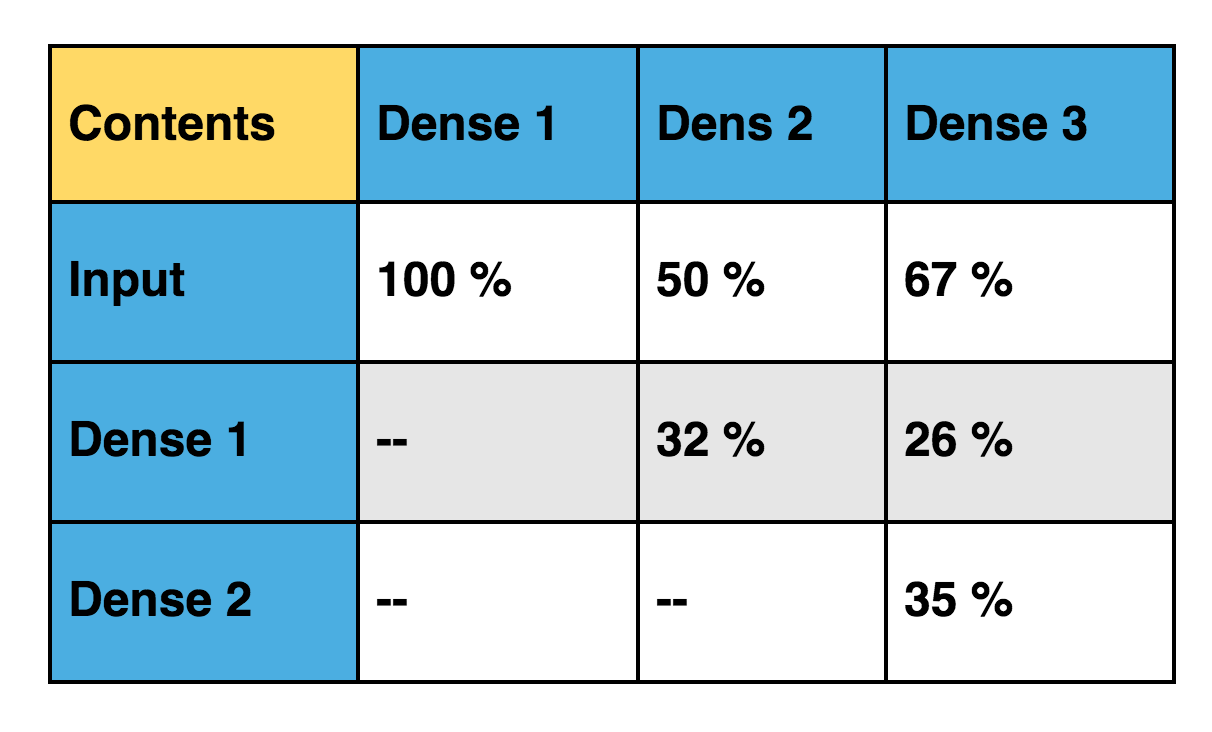
\includegraphics[scale=0.13]{SampleTable.png}
   \captionof{figure}{Sample Information Transfer Table}
   \label{fig:DSC.png}
\end{minipage}

\subsubsection{Pruning}
\begin{figure}[h!]
\centering
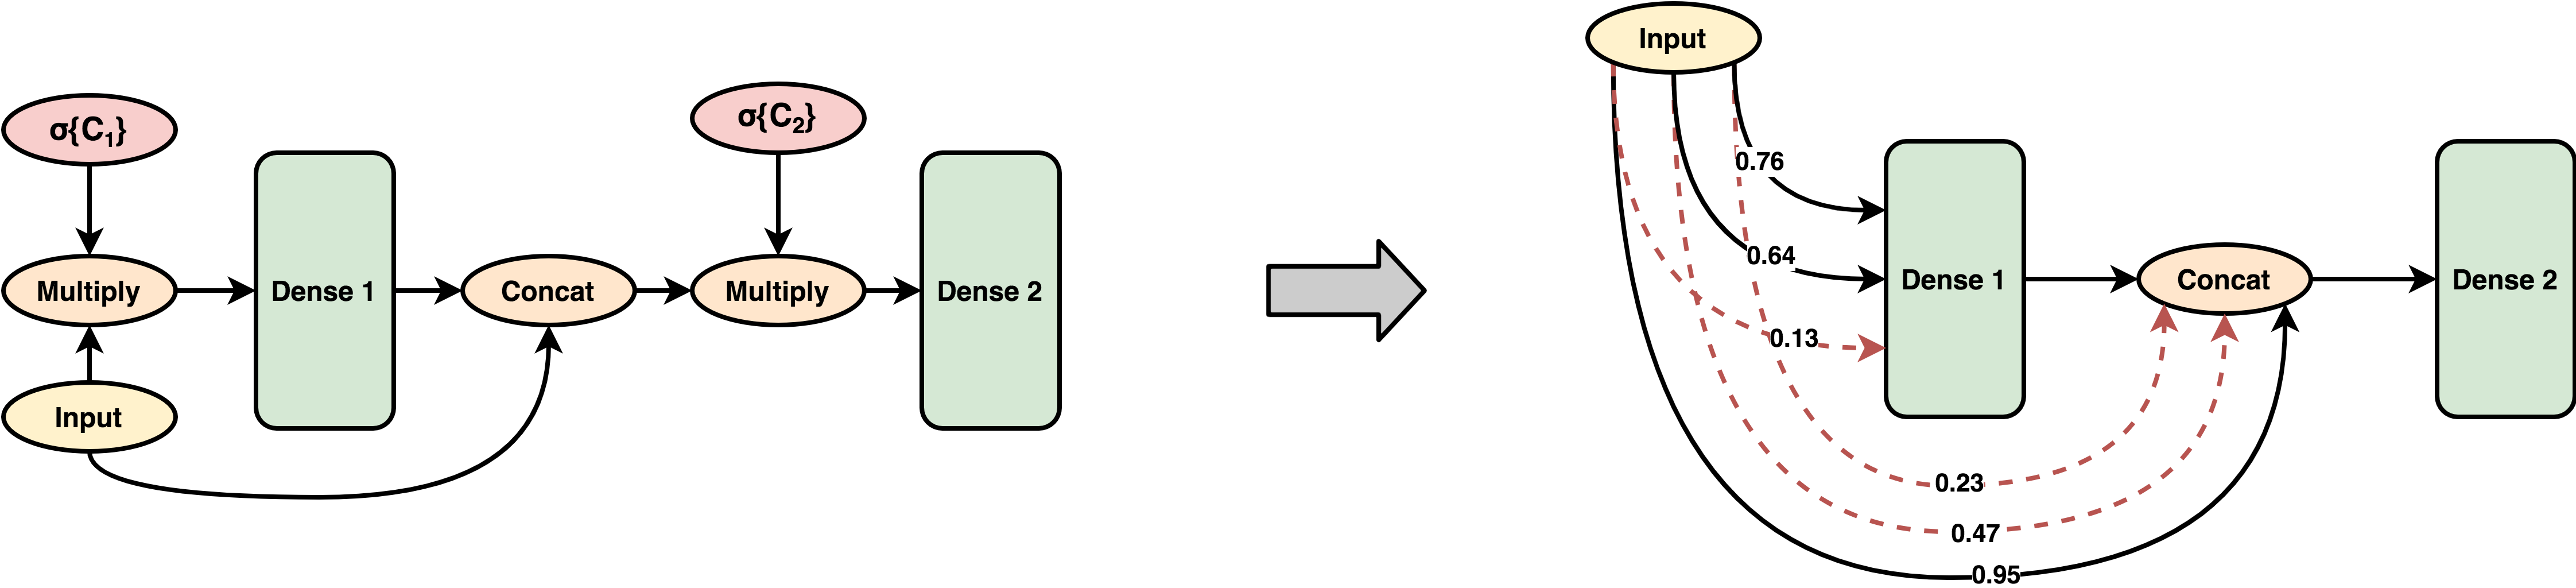
\includegraphics[scale=0.1]{Pruning.png}
\caption{Pruning}
\label{fig:infotransfer}
\end{figure}

\section{Experiments}
\label{sec:others}
\lipsum[8] \cite{kour2014real,kour2014fast} and see \cite{hadash2018estimate}.

The documentation for \verb+natbib+ may be found at
\begin{center}
  \url{http://mirrors.ctan.org/macros/latex/contrib/natbib/natnotes.pdf}
\end{center}
Of note is the command \verb+\citet+, which produces citations
appropriate for use in inline text.  For example,
\begin{verbatim}
   \citet{hasselmo} investigated\dots
\end{verbatim}
produces
\begin{quote}
  Hasselmo, et al.\ (1995) investigated\dots
\end{quote}

\begin{center}
  \url{https://www.ctan.org/pkg/booktabs}
\end{center}


\subsection{Figures}
\lipsum[10] 
See Figure \ref{fig:fig1}. Here is how you add footnotes. \footnote{Sample of the first footnote.}
\lipsum[11] 

\begin{figure}
  \centering
  \fbox{\rule[-.5cm]{4cm}{4cm} \rule[-.5cm]{4cm}{0cm}}
  \caption{Sample figure caption.}
  \label{fig:SimpleFFN.png}
\end{figure}

\subsection{Tables}
\lipsum[12]
See awesome Table~\ref{tab:table}.

% \begin{table}
%  \caption{Results}
%   \centering
%   \begin{tabular}{lll}
%     \toprule
%     \multicolumn{2}{c}{Part}                   \\
%     \cmidrule(r){1-2}
%     Model     & Parameters     & Dataset ($\mu$m) \\
%     \midrule
%     Dendrite & Input terminal  & $\sim$100     \\
%     Axon     & Output terminal & $\sim$10      \\
%     Soma     & Cell body       & up to $10^6$  \\
%     \bottomrule
%   \end{tabular}
%   \label{tab:table}
% \end{table}

% Please add the following required packages to your document preamble:
% Please add the following required packages to your document preamble:
% \usepackage{booktabs}
% \usepackage{multirow}
\begin{table}[]
\centering
\begin{tabular}{@{}llllllll@{}}
\toprule
\multirow{2}{*}{Model}      & \multirow{2}{*}{Parameter} & \multirow{2}{*}{Dataset} & \multicolumn{2}{l}{Train}       & \multicolumn{2}{l}{Test} & \multirow{2}{*}{Time Elapsed} \\ \cmidrule(lr){4-7}
                            &                            &                          & Accuracy @ Steps & Loss @ Steps & Accuracy      & Loss     &                               \\ \cmidrule(r){1-3} \cmidrule(l){8-8} 
\multirow{3}{*}{Linear FFN} & \multirow{3}{*}{84640}     & MNIST                    &                  &              &               &          &                               \\
                            &                            & FashionMNIST             &                  &              &               &          &                               \\
                            &                            & CIFAR-10                 &                  &              &               &          &                               \\
                            &                            &                          &                  &              &               &          &                               \\
GSC                         & 132100                     & MNIST                    &                  &              &               &          &                               \\
                            &                            & FashionMNIST             &                  &              &               &          &                               \\
                            &                            & CIFAR-10                 &                  &              &               &          &                               \\
                            &                            &                          &                  &              &               &          &                               \\
DSC                         & 133034                     & MNIST                    &                  &              &               &          &                               \\
                            &                            & FashionMNIST             &                  &              &               &          &                               \\
                            &                            & CIFAR-10                 &                  &              &               &          &                               \\
                            &                            &                          &                  &              &               &          &                               \\
DSC-10p                     & 24654                      & MNIST                    &                  &              &               &          &                               \\
                            &                            & FashionMNIST             &                  &              &               &          &                               \\
                            &                            & CIFAR-10                 &                  &              &               &          &                               \\ \bottomrule
\end{tabular}
\caption{100\% Data}
\label{tab:my-table}
\end{table}



\begin{figure}[h!]
\centering
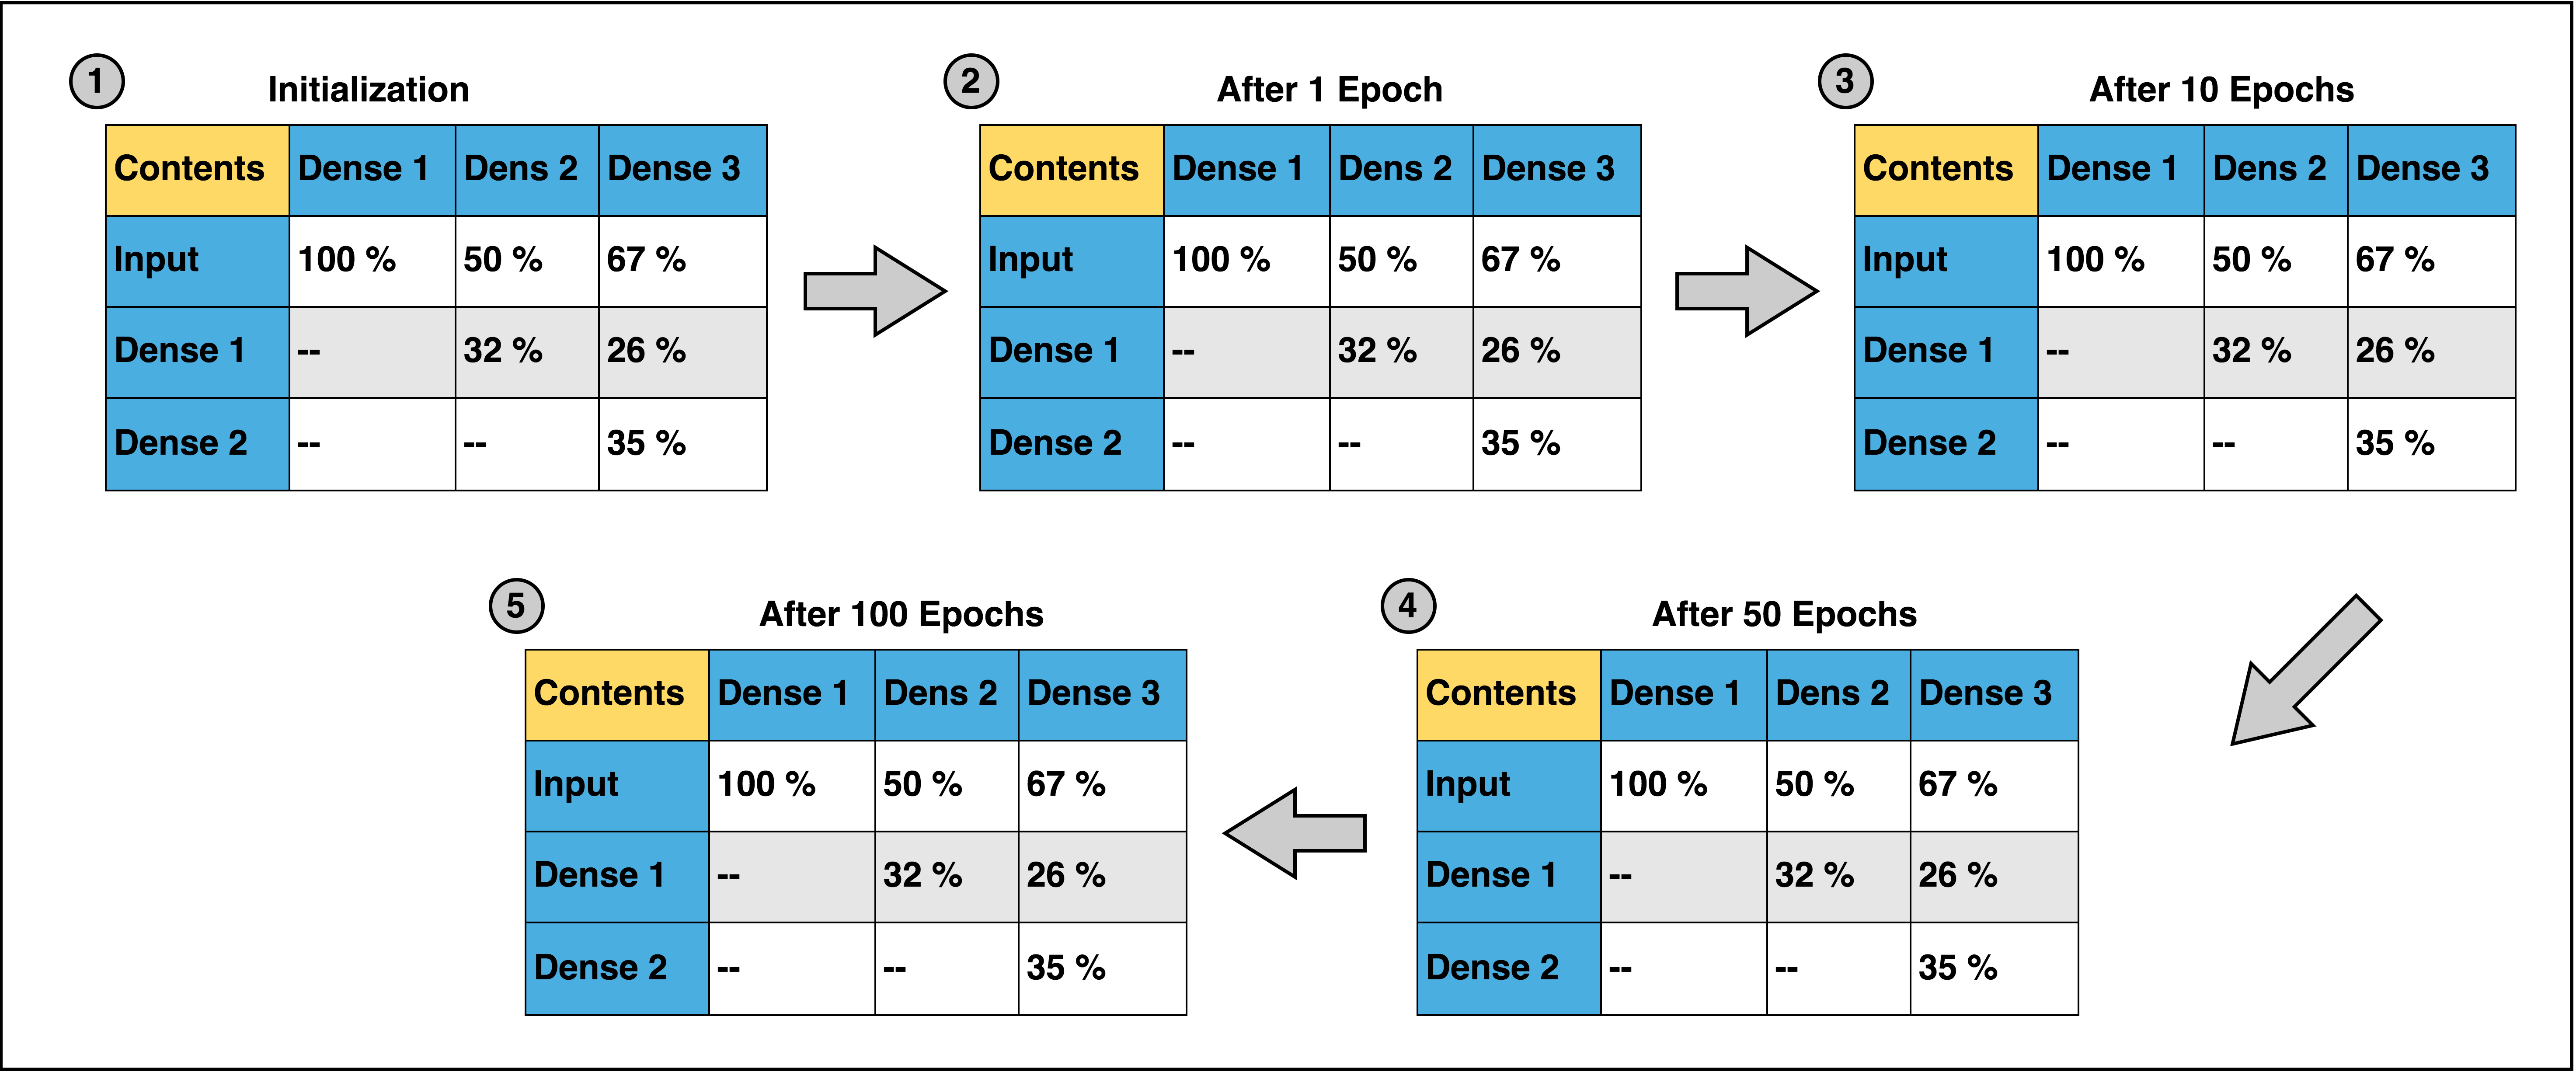
\includegraphics[scale=0.08]{InfoTransfer.png}
\caption{Information Transfer}
\label{fig:infotransfer}
\end{figure}


\subsection{Lists}
\begin{itemize}
\item Lorem ipsum dolor sit amet
\item consectetur adipiscing elit. 
\item Aliquam dignissim blandit est, in dictum tortor gravida eget. In ac rutrum magna.
\end{itemize}


\section{Conclusion}



\bibliographystyle{unsrt}  
\bibliography{references}
%\bibliography{references}  %%% Remove comment to use the external .bib file (using bibtex).
%%% and comment out the ``thebibliography'' section.


%%% Comment out this section when you \bibliography{references} is enabled.
% \begin{thebibliography}{1}

% \bibitem{kour2014real}
% George Kour and Raid Saabne.
% \newblock Real-time segmentation of on-line handwritten arabic script.
% \newblock In {\em Frontiers in Handwriting Recognition (ICFHR), 2014 14th
%   International Conference on}, pages 417--422. IEEE, 2014.

% \bibitem{kour2014fast}
% George Kour and Raid Saabne.
% \newblock Fast classification of handwritten on-line arabic characters.
% \newblock In {\em Soft Computing and Pattern Recognition (SoCPaR), 2014 6th
%   International Conference of}, pages 312--318. IEEE, 2014.

% \bibitem{hadash2018estimate}
% Guy Hadash, Einat Kermany, Boaz Carmeli, Ofer Lavi, George Kour, and Alon
%   Jacovi.
% \newblock Estimate and replace: A novel approach to integrating deep neural
%   networks with existing applications.
% \newblock {\em arXiv preprint arXiv:1804.09028}, 2018.

% \end{thebibliography}


\end{document}


